\chapter{Experiments and Results}\label{chapter:experiments}


\section{Dataset Overview}\label{section:experiments_dataset}

The set of input data for testing of the implemented system consisted of 34 piano recordings of various scales and intervals. The files were converted to WAV file format to address the limitations of the used libraries. Below is a more detailed overview:

\begin{itemize}
	\item A-major scale played fast and slow in ascending and descending order, starting from $A_3$
	\item A-minor scale played fast and slow in ascending and descending order in three modes: natural, harmonic and melodic, starting from $A_3$
	\item C-major scale played fast and slow in ascending and descending order, starting from $C_4$
	\item C-major scale, where each note is repeated 3 times, in ascending order in four variants: starting from $C_3$, $C_4$, $C_5$ and $C_6$
	\item D-major scale played fast and slow in ascending and descending order, starting from $D_4$
	\item E-major scale played fast and slow in ascending and descending order, starting from $E_4$
	\item E-minor scale played fast and slow in ascending and descending order in three modes: natural, harmonic and melodic, starting from $E_4$
	\item F-major scale played fast and slow in ascending and descending order, starting from $F_4$
	\item G-major scale played fast and slow in ascending and descending order, starting from $G_4$
	\item H-major scale played fast and slow in ascending and descending order, starting from $H_4$
	\item Perfect melodic fourths, where the lower notes are in range starting from $C_3$ and ending at $C_6$, in ascending order
	\item Perfect melodic octaves, where the lower notes are in range starting from $C_3$ and ending at $F_5$, in ascending order
	\item All semitones (or all keys one after another), starting from $C_4$ and ending at $H_5$, in ascending order
	\item All semitones (or all keys one after another), starting from $C_2$ and ending at $H_3$, in ascending order
\end{itemize}

\section{Experiments with White Noise}

The first set of experiments involved experiments with white noise levels. The noise level was an input parameter of the CASA system that was used before the peripheral analysis stage to modify the input sound. The functionality for combining sounds was provided by the \textit{brian2hears} \cite{brian2hears} package, and the noise level parameter was used as the amplitude of the white noise sound wave, which was then added to the input sound wave. The set of values for the noise level parameter was as follows: $\left\{0;~0.005;~0.01;~0.02;~0.04\right\}$. The results are shown on figure \ref{img:white_noise_experiments}.\\

On the figure, the first row depicts the results for the input sound without artificially added white noise, and each next row shows the results for different noise levels. When comparing the cochleagrams, the rising amounts of background noise can be clearly seen. From the resulting masking, it can be observed that the model began to lose the quality of source separation when the noise level was around $0.02$, which is clearly a major amount of randomness in the input, and can be well heard by a human listener. Given the simplicity of the algorithm for the segmentation-and-grouping stage, the outcomes can be considered a success.

\begin{figure}[t]
	\centering
	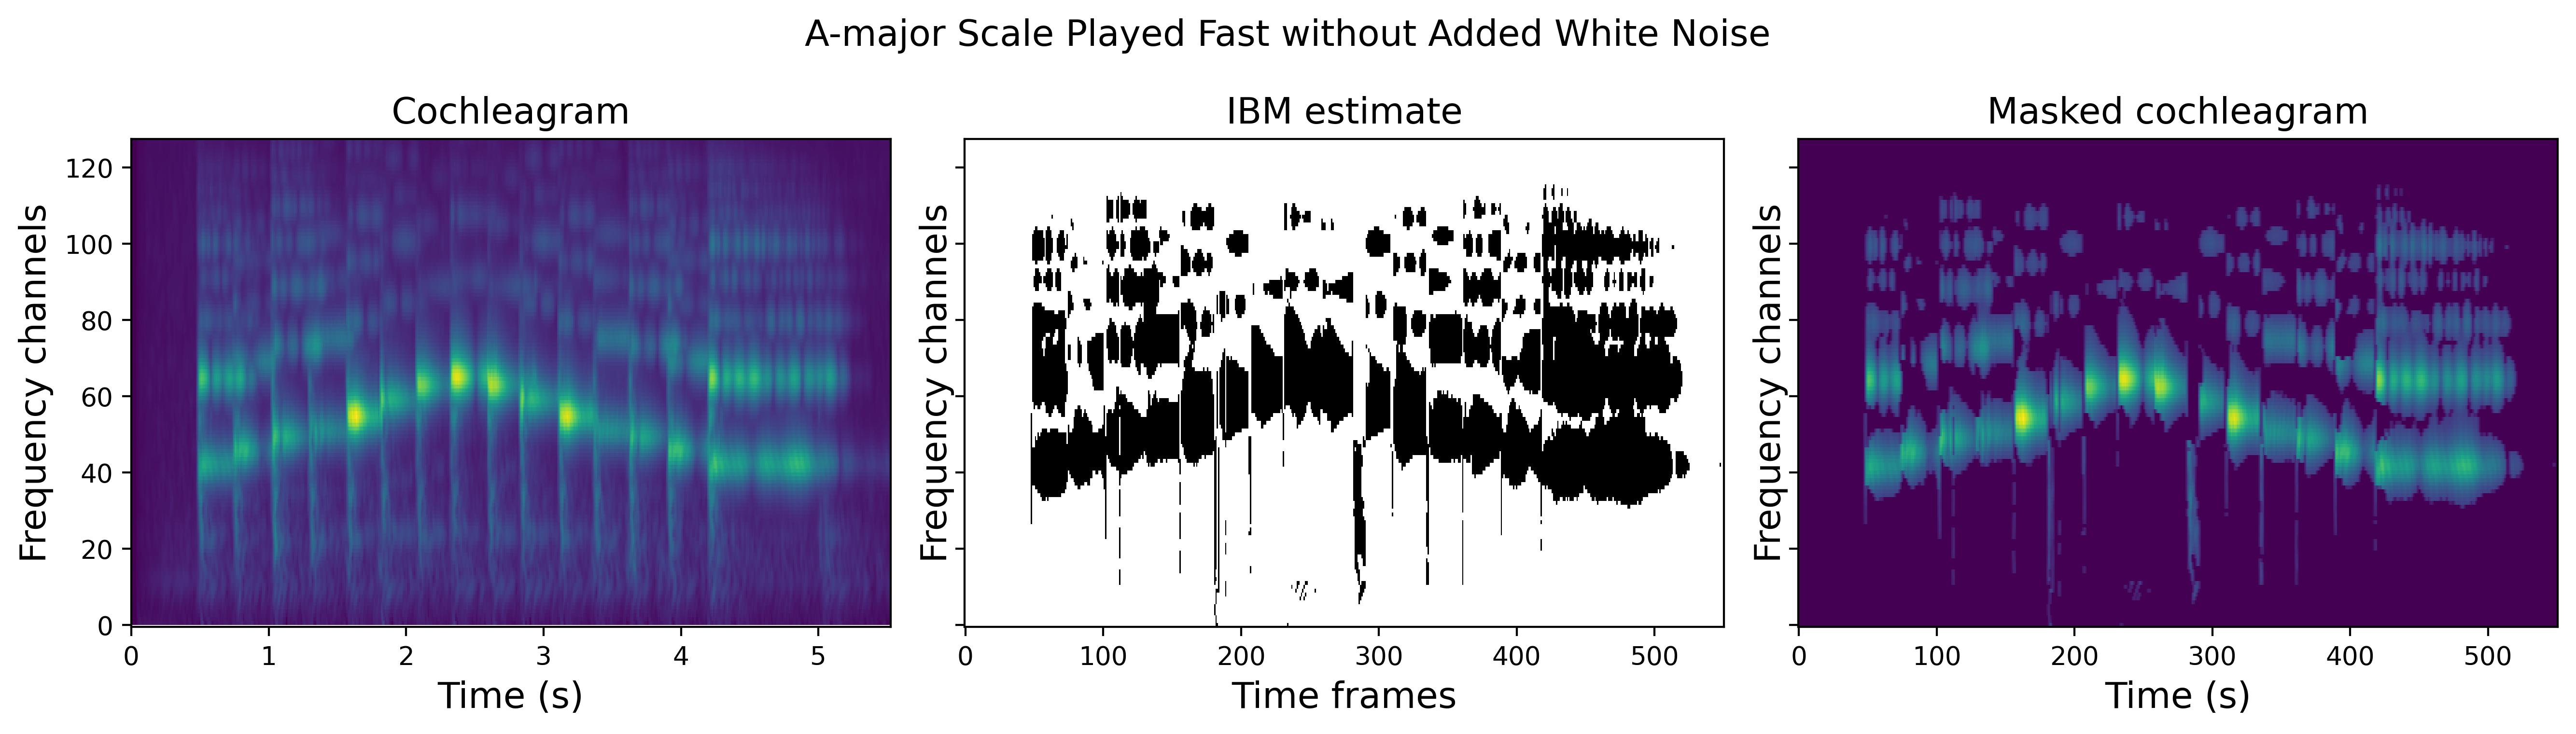
\includegraphics[width=\textwidth]{include/experiments_white_noise_A-major_0.jpg}
	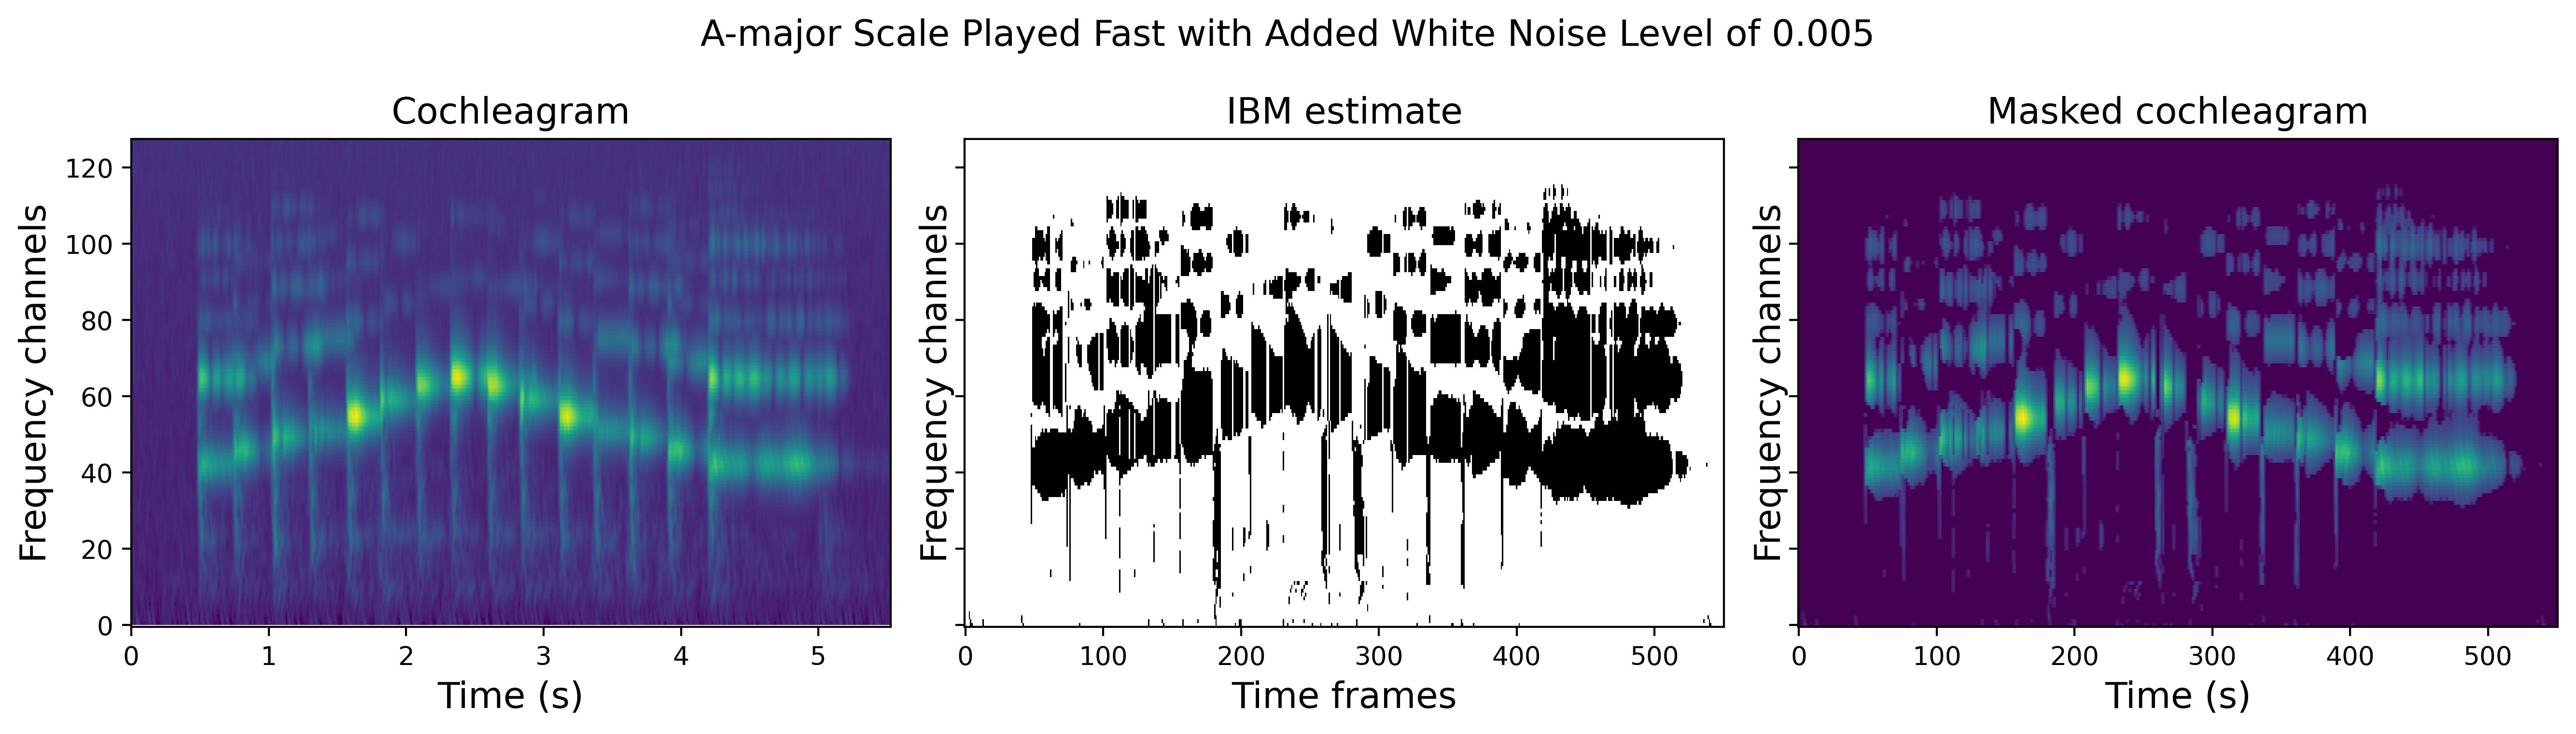
\includegraphics[width=\textwidth]{include/experiments_white_noise_A-major_0,005.jpg}
	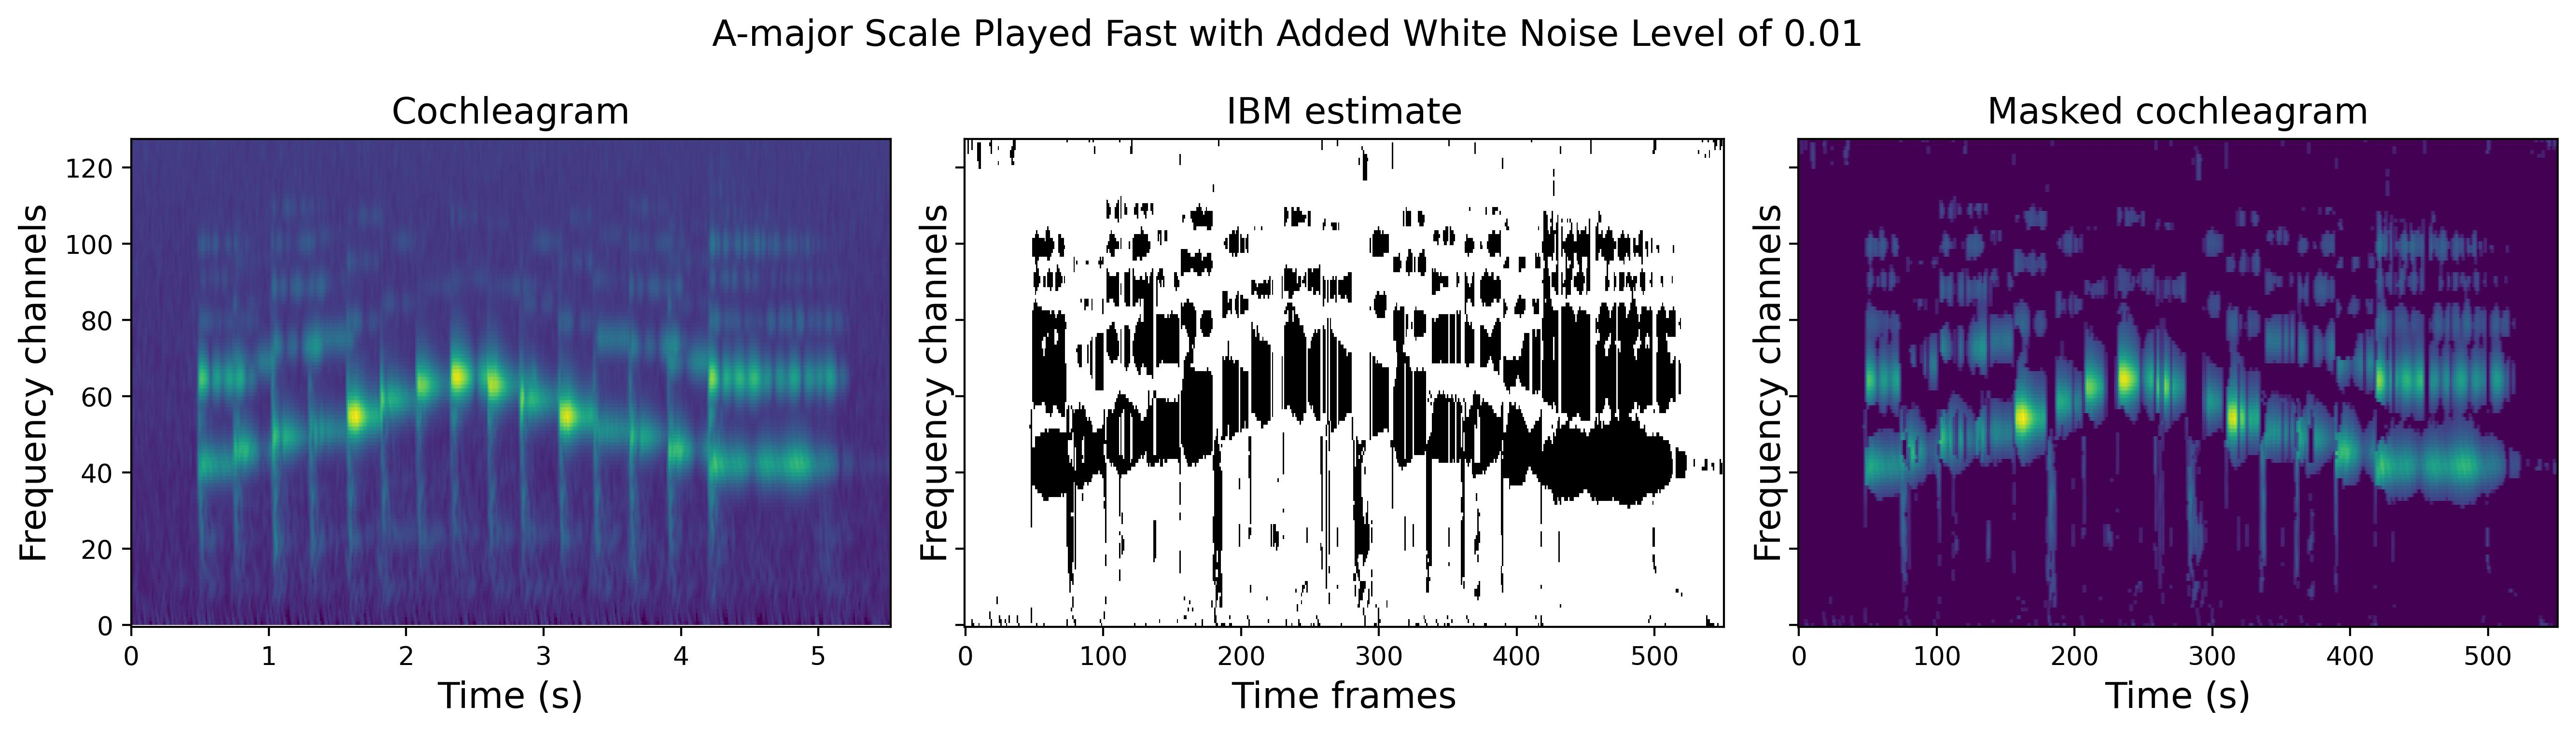
\includegraphics[width=\textwidth]{include/experiments_white_noise_A-major_0,01.jpg}
	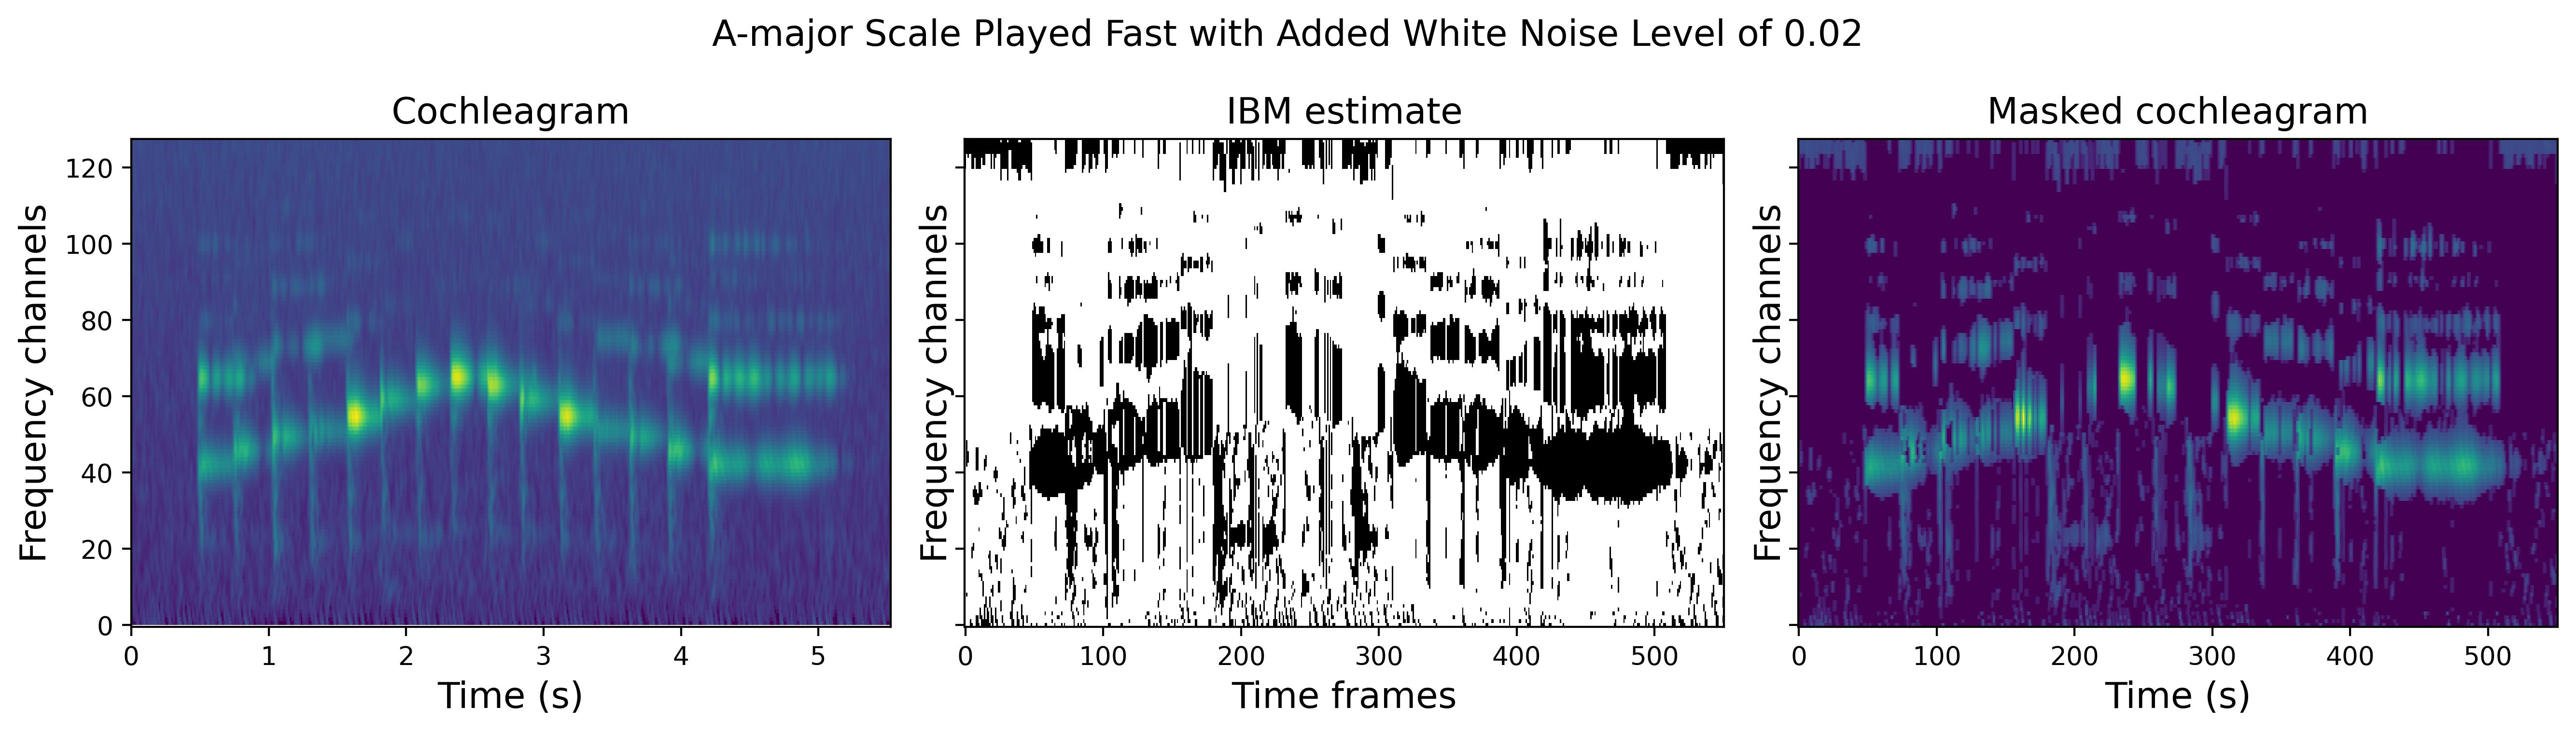
\includegraphics[width=\textwidth]{include/experiments_white_noise_A-major_0,02.jpg}
	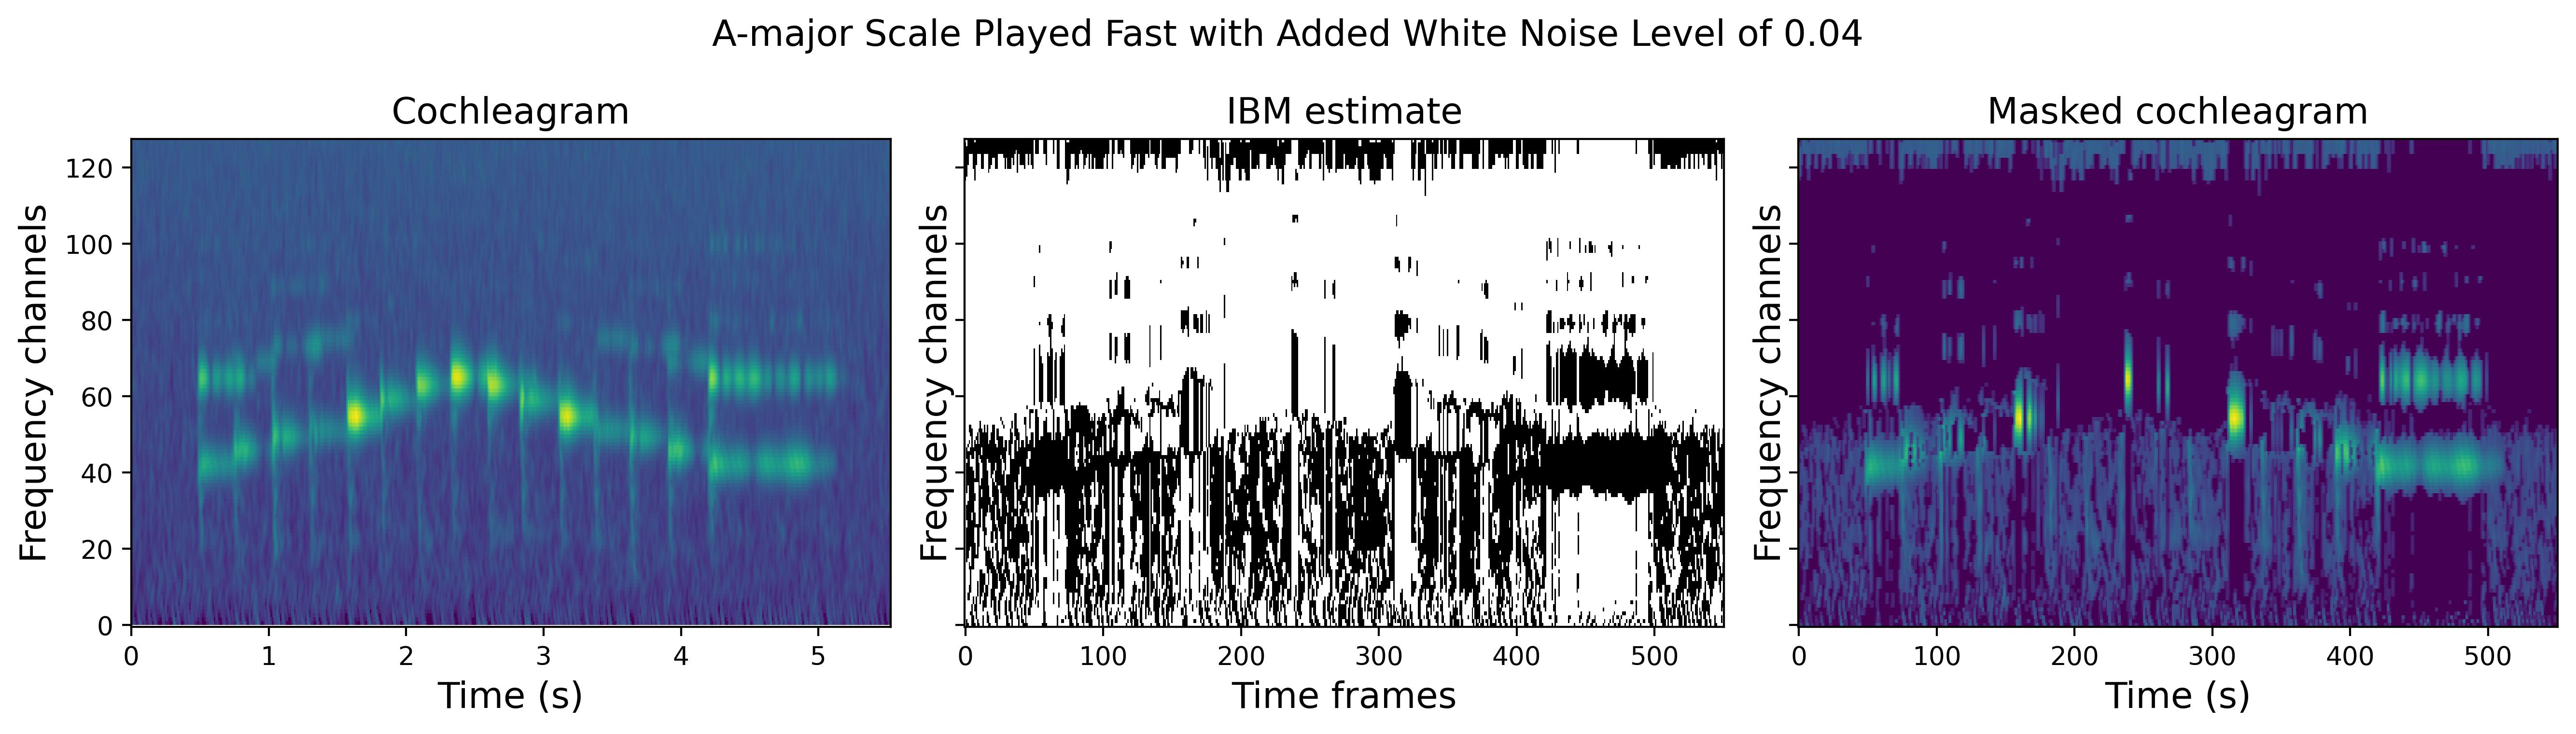
\includegraphics[width=\textwidth]{include/experiments_white_noise_A-major_0,04.jpg}
	\caption[Results of experiments with white noise levels]{Results of the experiments with white noise levels for A-major scale played fast. In each row, the first image is a cochleagram of the input sound, the second is the estimated IBM, and the third is the masked cochleagram.}
	\label{img:white_noise_experiments}
\end{figure}

\section{Other Experiments}